%\cleardoublepage
\phantomsection
%\tableofcontents
\section{Motivation}
 
  Over the last five decades the requirement for supersonic and hypersonic propulsion has grown considerably. Prediction of thermoacoustic oscillations gained importance in order to run rocket engines and gas turbines properly. This motivation requires to being capable of solving complicated mathematical models by utilizing adjoint methods.
  
  \section{Mathematical Model}
  
  1D thermoacoustic model has been considered. Mean flow has been set to zero. As can be seen in Figure \ref{fig:model}, open ended elongated tube from 0 to X containing gas at following parameters;
  \begin{itemize}
	\item{Uniform density, $\overline{\rho}$}
	\item{Uniform pressure, $\overline{p}$}
	\item{Ratio of specific heats, $\gamma$}
	\item{Velocity, $u$}
	\item{Pressure, $p$}  
\end{itemize}  
\begin{figure}[!htb]
	
	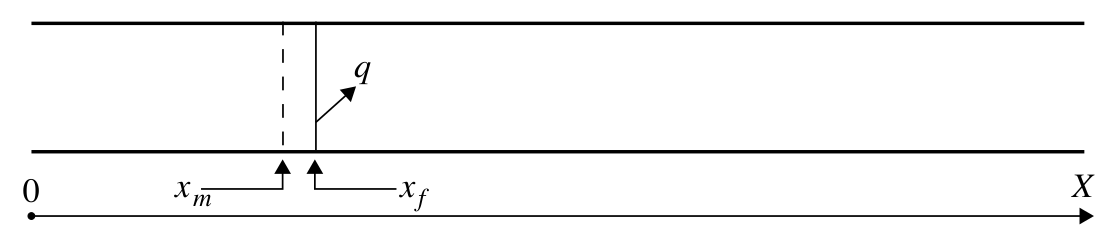
\includegraphics[width=\textwidth]{model.png}
	\caption{Diagram of the open-ended tube extending from 0 (upstream) to X (downstream). The heat
		release, q, occurs at position x f and is a function of the acoustic velocity at x m . The mean flow,
		which is defined as positive in the positive x-direction, is set to zero.}
	\label{fig:model}
	
\end{figure}

%\pagebreak
  





\subsection{Governing Equations}

The 1D acoustic energy and momentum equations are;

\begin{equation}
\overline{\rho}\frac{\partial u}{\partial t}+
\frac{\partial p}{\partial x}=0
\end{equation}

\begin{equation}
\frac{\partial p}{\partial t}+
\gamma \overline{p} \frac{\partial u}{\partial x}=(\gamma-1)q\delta_D (x-x_f)
\end{equation}
  
  
  
  Heat release rate $q(t)=nu(x_m,t_\tau) [W/m^2] $ is placed at $x=x_f$, where $n [J/m^3]$ is a real constant, $\tau$ is time delay, $x_m$ is the measurement position of $u$. Mean
  density drop across the heat source, viscous and thermal dissipations have been neglected. 
  
  $\delta$ is the Dirac delta. Reference length, reference speed and reference pressure are defined as $L_{ref}=X$, $U_{ref}=\overline{c}$ and $P_{ref}=\overline{p}$, respectively.Dimensionless acoustic energy and momentum equations are stated as follows;
  
  \begin{equation}
  \gamma \frac{\partial u}{\partial t}+
  \frac{\partial p}{\partial x}=0
  \label{eq:nondim1}
  \end{equation}
  
  \begin{equation}
  \frac{\partial p}{\partial t}+
  \gamma \frac{\partial u}{\partial x}=(\gamma-1)q\delta_D (x-x_f)
  \label{eq:nondim2}
  \end{equation}
  